\documentclass[aspectratio=169, 11pt]{beamer}

% ── Theme & Colors ──────────────────────────────────────────────
\usetheme{Madrid}
\usecolortheme{default}
\definecolor{asnublue}{RGB}{0,80,158}
\definecolor{asnugray}{RGB}{100,100,100}
\setbeamercolor{structure}{fg=asnublue}
\setbeamercolor{frametitle}{bg=asnublue, fg=white}
\setbeamercolor{title}{bg=asnublue, fg=white}
\setbeamercolor{block title}{bg=asnublue, fg=white}
\setbeamercolor{block body}{bg=asnublue!5}
\setbeamertemplate{navigation symbols}{}
\setbeamertemplate{footline}{%
  \leavevmode\hbox{%
    \begin{beamercolorbox}[wd=.33\paperwidth,ht=2.5ex,dp=1ex,center]{author in head/foot}%
      \usebeamerfont{author in head/foot}\insertshortauthor
    \end{beamercolorbox}%
    \begin{beamercolorbox}[wd=.34\paperwidth,ht=2.5ex,dp=1ex,center]{title in head/foot}%
      \usebeamerfont{title in head/foot}\insertshorttitle
    \end{beamercolorbox}%
    \begin{beamercolorbox}[wd=.33\paperwidth,ht=2.5ex,dp=1ex,right]{date in head/foot}%
      \usebeamerfont{date in head/foot}\insertframenumber{} / \inserttotalframenumber\hspace*{2ex}
    \end{beamercolorbox}}%
}

% ── Packages ────────────────────────────────────────────────────
\usepackage{booktabs}
\usepackage{graphicx}
\usepackage{tikz}
\usetikzlibrary{arrows.meta, positioning, shapes, fit, calc, decorations.pathreplacing}
\usepackage{amsmath}
\usepackage{multirow}
\usepackage{adjustbox}
\usepackage{colortbl}

% ── Title ───────────────────────────────────────────────────────
\title[ASNU]{ASNU: Aggregated Social Network Unfolder}
\subtitle{Generating Realistic Synthetic Networks from Aggregate Demographic Data}
\author{Kamiel Gulpen}
\institute{PhD Research}
\date{\today}

\begin{document}

% ════════════════════════════════════════════════════════════════
%  TITLE
% ════════════════════════════════════════════════════════════════
\begin{frame}[plain]
  \titlepage
\end{frame}

% ════════════════════════════════════════════════════════════════
%  OUTLINE
% ════════════════════════════════════════════════════════════════
\begin{frame}{Outline}
  \tableofcontents
\end{frame}

% ════════════════════════════════════════════════════════════════
%  SECTION 1 — INTRODUCTION
% ════════════════════════════════════════════════════════════════
\section{Introduction}

\begin{frame}{Motivation}
  \begin{columns}[T]
    \begin{column}{0.55\textwidth}
      \textbf{The problem:}
      \begin{itemize}
        \item Agent-based models (ABMs) for epidemiology, policy analysis, and social simulation require \textbf{realistic contact networks}
        \item Individual-level interaction data is rarely available due to privacy and cost
        \item What \emph{is} available: \textbf{aggregate demographic statistics} (census, surveys)
      \end{itemize}
      \vspace{1em}
      \textbf{The gap:}
      \begin{itemize}
        \item Classic network models (ER, BA, SBM) generate from abstract parameters
        \item Existing synthetic population tools often lack network generation or require geospatial data
      \end{itemize}
    \end{column}
    \begin{column}{0.42\textwidth}
      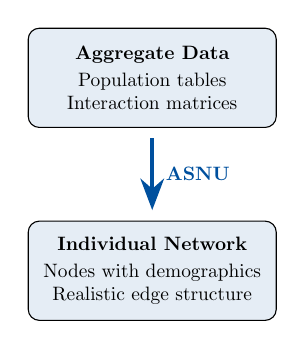
\begin{tikzpicture}[scale=0.7, every node/.style={scale=0.7}]
        % Aggregate data box
        \node[draw, rounded corners, fill=asnublue!10, minimum width=4.5cm, minimum height=1.8cm, align=center] (agg) at (0,3.5) {
          \textbf{Aggregate Data}\\[2pt]
          Population tables\\
          Interaction matrices
        };
        % Arrow
        \draw[-{Stealth[length=4mm]}, line width=1.5pt, asnublue] (0,2.4) -- node[right, xshift=3pt] {\textbf{ASNU}} (0,1.1);
        % Network
        \node[draw, rounded corners, fill=asnublue!10, minimum width=4.5cm, minimum height=1.8cm, align=center] (net) at (0,0) {
          \textbf{Individual Network}\\[2pt]
          Nodes with demographics\\
          Realistic edge structure
        };
      \end{tikzpicture}
    \end{column}
  \end{columns}
\end{frame}

\begin{frame}{Research Question}
  \begin{block}{Central Question}
    How can we \textbf{unfold} aggregated population-level interaction data into realistic individual-level social networks that preserve demographic structure and exhibit tunable topological properties?
  \end{block}
  \vspace{1em}
  \textbf{Requirements:}
  \begin{enumerate}
    \item Preserve group-level interaction counts from input data
    \item Support tunable network properties: preferential attachment, reciprocity, transitivity
    \item Generate community structure consistent with demographic mixing patterns
    \item Scale to large populations (millions of nodes)
    \item Support multiplex (layered) networks: household, family, neighborhood, work/school
  \end{enumerate}
\end{frame}

\begin{frame}{Classic Models and Their Limitations}
  \begin{table}
    \centering
    \small
    \begin{tabular}{@{}lcccc@{}}
      \toprule
      \textbf{Property} & \textbf{Erd\H{o}s--R\'enyi} & \textbf{Barab\'asi--Albert} & \textbf{SBM} & \textbf{ASNU} \\
      \midrule
      Input & $n, p$ & $n, m$ & Block matrix & \cellcolor{asnublue!10}\textbf{Real data} \\
      Degree distribution & Poisson & Power-law & Per-block & \cellcolor{asnublue!10}\textbf{Data-driven} \\
      Communities & \texttimes & \texttimes & \checkmark & \cellcolor{asnublue!10}\checkmark \\
      Directed edges & \texttimes & \texttimes & Optional & \cellcolor{asnublue!10}\checkmark \\
      Reciprocity & --- & --- & --- & \cellcolor{asnublue!10}\textbf{Tunable} \\
      Transitivity & $\approx 0$ & Low & Within-block & \cellcolor{asnublue!10}\textbf{Tunable} \\
      Multiplex & \texttimes & \texttimes & \texttimes & \cellcolor{asnublue!10}\checkmark \\
      Demographics & \texttimes & \texttimes & Block label & \cellcolor{asnublue!10}\textbf{Rich} \\
      \bottomrule
    \end{tabular}
  \end{table}
  \vspace{0.5em}
  \begin{center}
    \small Classic models answer: ``\emph{What does a network look like given abstract rules?}''\\
    ASNU answers: ``\emph{Given real population data, what could the actual network look like?}''
  \end{center}
\end{frame}

% ════════════════════════════════════════════════════════════════
%  SECTION 2 — DATA
% ════════════════════════════════════════════════════════════════
\section{Data}

\begin{frame}{Data Sources: Dutch Population Statistics}
  \begin{columns}[T]
    \begin{column}{0.48\textwidth}
      \textbf{Population Data}\\[4pt]
      Demographic group sizes from aggregated survey/census data.\\[6pt]
      \small
      \begin{tabular}{@{}llll r@{}}
        \toprule
        \textbf{Gender} & \textbf{Age} & \textbf{Ethn.} & \textbf{Edu.} & \textbf{$n$} \\
        \midrule
        Female & [20,30) & Other & 1 & 3\,870 \\
        Female & [20,30) & Other & 2 & 15\,730 \\
        Male & [50,60) & Native & 1 & 4\,911 \\
        Male & [0,20) & Native & 3 & 32\,450 \\
        \textvdots & \textvdots & \textvdots & \textvdots & \textvdots \\
        \bottomrule
      \end{tabular}
      \vspace{6pt}\\
      \textbf{85 demographic groups}\\
      $\approx$\,\textbf{5.7 million} total population
    \end{column}
    \begin{column}{0.50\textwidth}
      \textbf{Demographic Characteristics}\\[6pt]
      \begin{itemize}
        \item \textbf{Gender} (2): Male, Female
        \item \textbf{Age} (5): [0,20), [20,30), [30,40), [40,50), [50,60), 60+
        \item \textbf{Ethnicity} (3): Native, Moroccan, Other
        \item \textbf{Education} (3): Low, Medium, High
      \end{itemize}
      \vspace{0.8em}
      \begin{block}{Key Property}
        ASNU accepts \textbf{any} set of categorical characteristics --- the framework is not tied to specific demographic variables.
      \end{block}
    \end{column}
  \end{columns}
\end{frame}

\begin{frame}{Data Sources: Interaction Layers}
  \textbf{Four interaction layers} capture different social contexts:
  \vspace{0.3em}

  \begin{table}
    \centering
    \small
    \begin{tabular}{@{}l l r r@{}}
      \toprule
      \textbf{Layer} & \textbf{Description} & \textbf{Group Pairs} & \textbf{Context} \\
      \midrule
      \texttt{huishouden} & Household contacts & $\sim$8\,700 & Co-residence \\
      \texttt{familie} & Family contacts & $\sim$4\,200 & Kinship ties \\
      \texttt{buren} & Neighbor contacts & $\sim$24\,800 & Spatial proximity \\
      \texttt{werkschool} & Work/school contacts & $\sim$13\,800 & Occupational \\
      \bottomrule
    \end{tabular}
  \end{table}

  \vspace{0.5em}
  Each layer is a matrix of \textbf{aggregate interaction counts} between source--destination group pairs:

  \vspace{0.3em}
  \small
  \begin{tabular}{@{}llll|llll|r@{}}
    \toprule
    \multicolumn{4}{c|}{\textbf{Source Group}} & \multicolumn{4}{c|}{\textbf{Destination Group}} & \textbf{$n$} \\
    \textit{gender} & \textit{age} & \textit{edu} & \textit{ethn} & \textit{gender} & \textit{age} & \textit{edu} & \textit{ethn} & \\
    \midrule
    Male & [0,20) & 1 & Native & Male & [0,20) & 1 & Native & 14\,580 \\
    Male & [0,20) & 1 & Native & Male & [0,20) & 2 & Native & 360 \\
    Female & [30,40) & 2 & Other & Male & [40,50) & 3 & Native & 1\,245 \\
    \bottomrule
  \end{tabular}
\end{frame}

\begin{frame}{Data Structure: From Aggregate to Individual}
  \begin{center}
    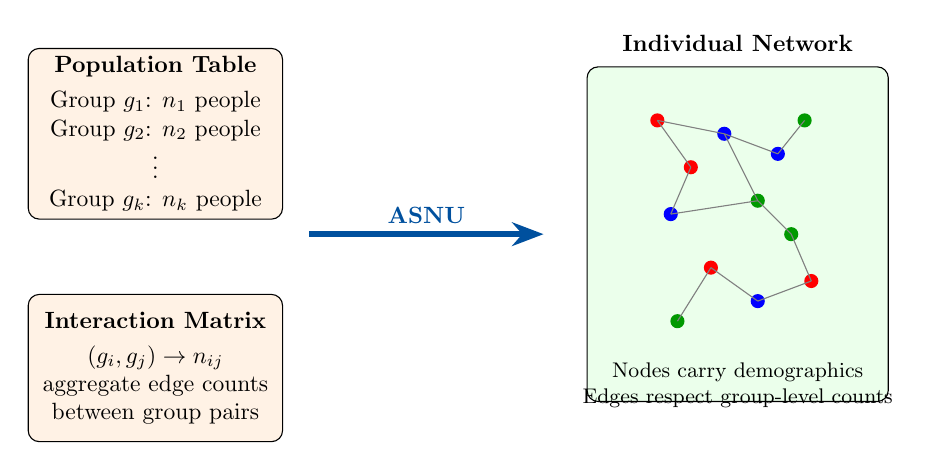
\begin{tikzpicture}[scale=0.85, every node/.style={scale=0.85}]
      % Left: aggregate
      \node[draw, rounded corners, fill=orange!10, minimum width=3.8cm, minimum height=2.2cm, align=center] (pop) at (-4.5,0) {
        \textbf{Population Table}\\[3pt]
        Group $g_1$: $n_1$ people\\
        Group $g_2$: $n_2$ people\\
        $\vdots$\\
        Group $g_k$: $n_k$ people
      };
      \node[draw, rounded corners, fill=orange!10, minimum width=3.8cm, minimum height=2.2cm, align=center] (int) at (-4.5,-3.5) {
        \textbf{Interaction Matrix}\\[3pt]
        $(g_i, g_j) \rightarrow n_{ij}$\\
        aggregate edge counts\\
        between group pairs
      };

      % Arrow
      \draw[-{Stealth[length=4mm]}, line width=2pt, asnublue] (-2.2,-1.5) -- node[above, sloped] {\textbf{ASNU}} (1.3,-1.5);

      % Right: individual network
      \node[draw, rounded corners, fill=green!8, minimum width=4.5cm, minimum height=5cm, align=center] (net) at (4.2,-1.5) {};
      \node[above] at (4.2,1.1) {\textbf{Individual Network}};

      % Draw some nodes with colors for groups
      \foreach \x/\y/\c in {3.0/0.2/red, 3.5/-0.5/red, 3.2/-1.2/blue, 4.0/0.0/blue, 4.8/-0.3/blue, 5.2/0.2/green!60!black, 4.5/-1.0/green!60!black, 3.8/-2.0/red, 4.5/-2.5/blue, 5.0/-1.5/green!60!black, 3.3/-2.8/green!60!black, 5.3/-2.2/red} {
        \fill[\c] (\x,\y) circle (3pt);
      }
      % Draw some edges
      \draw[gray, thin] (3.0,0.2) -- (3.5,-0.5);
      \draw[gray, thin] (3.5,-0.5) -- (3.2,-1.2);
      \draw[gray, thin] (4.0,0.0) -- (4.8,-0.3);
      \draw[gray, thin] (4.8,-0.3) -- (5.2,0.2);
      \draw[gray, thin] (4.5,-1.0) -- (5.0,-1.5);
      \draw[gray, thin] (3.0,0.2) -- (4.0,0.0);
      \draw[gray, thin] (3.8,-2.0) -- (4.5,-2.5);
      \draw[gray, thin] (4.5,-2.5) -- (5.3,-2.2);
      \draw[gray, thin] (3.3,-2.8) -- (3.8,-2.0);
      \draw[gray, thin] (3.2,-1.2) -- (4.5,-1.0);
      \draw[gray, thin] (5.0,-1.5) -- (5.3,-2.2);
      \draw[gray, thin] (4.0,0.0) -- (4.5,-1.0);

      \node[below, align=center, font=\small] at (4.2,-3.3) {
        Nodes carry demographics\\
        Edges respect group-level counts
      };
    \end{tikzpicture}
  \end{center}
\end{frame}

% ════════════════════════════════════════════════════════════════
%  SECTION 3 — FRAMEWORK
% ════════════════════════════════════════════════════════════════
\section{Framework}

\begin{frame}{ASNU Architecture Overview}
  \begin{center}
    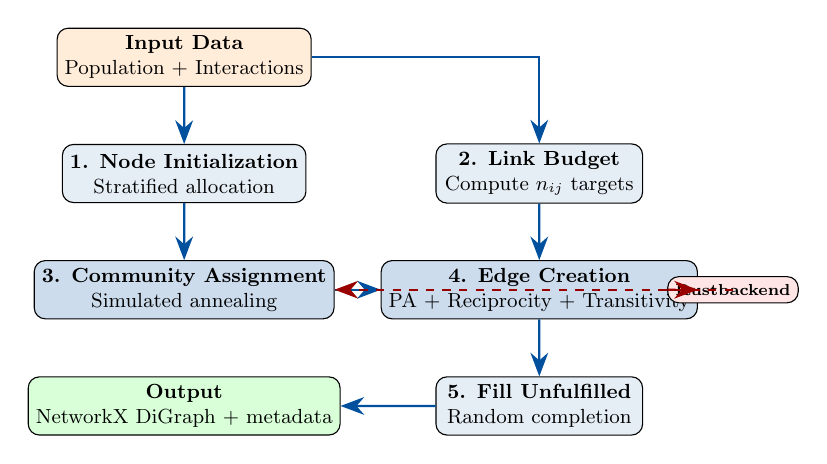
\begin{tikzpicture}[
      box/.style={draw, rounded corners, minimum width=3.2cm, minimum height=0.9cm, align=center, font=\small},
      arr/.style={-{Stealth[length=3mm]}, thick, asnublue},
      scale=0.82, every node/.style={scale=0.82}
    ]
      % Step 1
      \node[box, fill=orange!15] (input) at (0,0) {\textbf{Input Data}\\Population + Interactions};

      % Step 2
      \node[box, fill=asnublue!10] (nodes) at (0,-1.8) {\textbf{1. Node Initialization}\\Stratified allocation};

      % Step 3
      \node[box, fill=asnublue!10] (budget) at (5.5,-1.8) {\textbf{2. Link Budget}\\Compute $n_{ij}$ targets};

      % Step 4
      \node[box, fill=asnublue!20] (comm) at (0,-3.6) {\textbf{3. Community Assignment}\\Simulated annealing};

      % Step 5
      \node[box, fill=asnublue!20] (edges) at (5.5,-3.6) {\textbf{4. Edge Creation}\\PA + Reciprocity + Transitivity};

      % Step 6
      \node[box, fill=asnublue!10] (fill) at (5.5,-5.4) {\textbf{5. Fill Unfulfilled}\\Random completion};

      % Step 7
      \node[box, fill=green!15] (output) at (0,-5.4) {\textbf{Output}\\NetworkX DiGraph + metadata};

      % Rust badge
      \node[draw, rounded corners, fill=red!10, font=\scriptsize\bfseries] (rust) at (8.5,-3.6) {Rust\\backend};

      % Arrows
      \draw[arr] (input) -- (nodes);
      \draw[arr] (input.east) -| (budget);
      \draw[arr] (nodes) -- (comm);
      \draw[arr] (budget) -- (edges);
      \draw[arr] (comm.east) -- (edges.west);
      \draw[arr] (edges) -- (fill);
      \draw[arr] (fill) -- (output);
      \draw[arr, red!60!black, dashed] (rust) -- (edges);
      \draw[arr, red!60!black, dashed] (rust) |- (comm);
    \end{tikzpicture}
  \end{center}
\end{frame}

\begin{frame}{Step 1: Node Initialization --- Stratified Allocation}
  \begin{block}{Goal}
    Create $N' = \text{scale} \times N$ nodes preserving the demographic distribution of the original population.
  \end{block}
  \vspace{0.5em}
  \textbf{Stratified allocation algorithm:}
  \begin{enumerate}
    \item For each group $g_i$ with population $n_i$, compute target: $n'_i = \lfloor \text{scale} \times n_i \rfloor$
    \item Distribute remainder $r = N' - \sum n'_i$ to groups with the largest fractional parts
    \item Assign demographic attributes to each node
  \end{enumerate}

  \vspace{0.5em}
  \textbf{Example} (scale = 0.01, $N = 5.7$M):
  \begin{table}
    \centering\small
    \begin{tabular}{@{}l r r r@{}}
      \toprule
      \textbf{Group} & \textbf{Original $n$} & \textbf{Scaled $n'$} & \textbf{Proportion preserved} \\
      \midrule
      Male, [20,30), Native, Edu-2 & 24\,500 & 245 & \checkmark \\
      Female, [50,60), Other, Edu-1 & 3\,870 & 39 & \checkmark \\
      \bottomrule
    \end{tabular}
  \end{table}
\end{frame}

\begin{frame}{Step 2: Community Assignment via Simulated Annealing}
  \begin{columns}[T]
    \begin{column}{0.55\textwidth}
      \textbf{Agent-based assignment:} each node chooses a community to minimize distance from its \textit{ideal link distribution}.\\[6pt]

      For node $v$ in group $g$, and community $c$:
      \[
        d(v, c) = \sum_{g'} \left| P_{\text{ideal}}(g, g') - P_{\text{actual}}(c, g') \right|
      \]

      \textbf{Simulated annealing schedule:}
      \begin{itemize}
        \item High temperature $\rightarrow$ stochastic exploration
        \item Low temperature $\rightarrow$ greedy exploitation
        \item Probability: $P(\text{select } c) \propto e^{-d(v,c) / T}$
      \end{itemize}

      \vspace{0.5em}
      \textbf{Community size distributions:}\\
      Natural $|$ Uniform $|$ Power-law
    \end{column}
    \begin{column}{0.42\textwidth}
      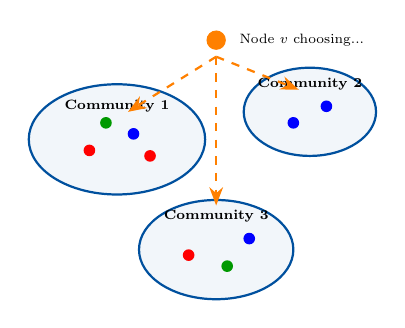
\begin{tikzpicture}[scale=0.7, every node/.style={scale=0.7}]
        % Communities
        \draw[thick, asnublue, fill=asnublue!5] (0,0) ellipse (1.6 and 1);
        \draw[thick, asnublue, fill=asnublue!5] (3.5,0.5) ellipse (1.2 and 0.8);
        \draw[thick, asnublue, fill=asnublue!5] (1.8,-2) ellipse (1.4 and 0.9);

        \node[font=\scriptsize\bfseries] at (0,0.6) {Community 1};
        \node[font=\scriptsize\bfseries] at (3.5,1.0) {Community 2};
        \node[font=\scriptsize\bfseries] at (1.8,-1.4) {Community 3};

        % Nodes
        \fill[red] (-0.5,-0.2) circle (3pt);
        \fill[blue] (0.3,0.1) circle (3pt);
        \fill[red] (0.6,-0.3) circle (3pt);
        \fill[green!60!black] (-0.2,0.3) circle (3pt);
        \fill[blue] (3.2,0.3) circle (3pt);
        \fill[blue] (3.8,0.6) circle (3pt);
        \fill[red] (1.3,-2.1) circle (3pt);
        \fill[green!60!black] (2.0,-2.3) circle (3pt);
        \fill[blue] (2.4,-1.8) circle (3pt);

        % New node choosing
        \fill[orange] (1.8,1.8) circle (5pt);
        \node[right, font=\scriptsize] at (2.1,1.8) {Node $v$ choosing...};
        \draw[-{Stealth}, thick, orange, dashed] (1.8,1.5) -- (0.2,0.5);
        \draw[-{Stealth}, thick, orange, dashed] (1.8,1.5) -- (3.3,0.9);
        \draw[-{Stealth}, thick, orange, dashed] (1.8,1.5) -- (1.8,-1.2);
      \end{tikzpicture}
    \end{column}
  \end{columns}
\end{frame}

\begin{frame}{Step 3: Edge Creation Mechanisms}
  Three tunable mechanisms operate \textbf{simultaneously} during edge creation:

  \vspace{0.5em}
  \begin{columns}[T]
    \begin{column}{0.32\textwidth}
      \begin{block}{Preferential Attachment}
        Popular nodes attract more edges.\\[4pt]
        \small
        \begin{itemize}
          \item Popularity pool: subset of destination nodes
          \item Smaller pool $\rightarrow$ stronger PA
          \item Scope: \textit{local} (within community) or \textit{global}
        \end{itemize}
      \end{block}
    \end{column}
    \begin{column}{0.32\textwidth}
      \begin{block}{Reciprocity}
        Mutual connections.\\[4pt]
        \small
        \begin{itemize}
          \item $P(\text{add } v \rightarrow u \mid u \rightarrow v) = r$
          \item Controlled by parameter $r \in [0,1]$
          \item Respects link budget constraints
        \end{itemize}
      \end{block}
    \end{column}
    \begin{column}{0.32\textwidth}
      \begin{block}{Transitivity}
        Friend-of-a-friend closure.\\[4pt]
        \small
        \begin{itemize}
          \item $P(\text{add } u \rightarrow w \mid u \rightarrow v, v \rightarrow w) = t$
          \item Creates clustering coefficient
          \item Parameter $t \in [0,1]$
        \end{itemize}
      \end{block}
    \end{column}
  \end{columns}

  \vspace{1em}
  \begin{block}{Bridge Probability}
    Controls inter-community edges: with probability $b$, an edge targets a \textbf{neighboring community} instead of the node's own community. This prevents isolated clusters.
  \end{block}
\end{frame}

\begin{frame}{Multiplex Network Generation}
  ASNU generates \textbf{hierarchical multiplex networks} where layers build upon each other:

  \begin{center}
    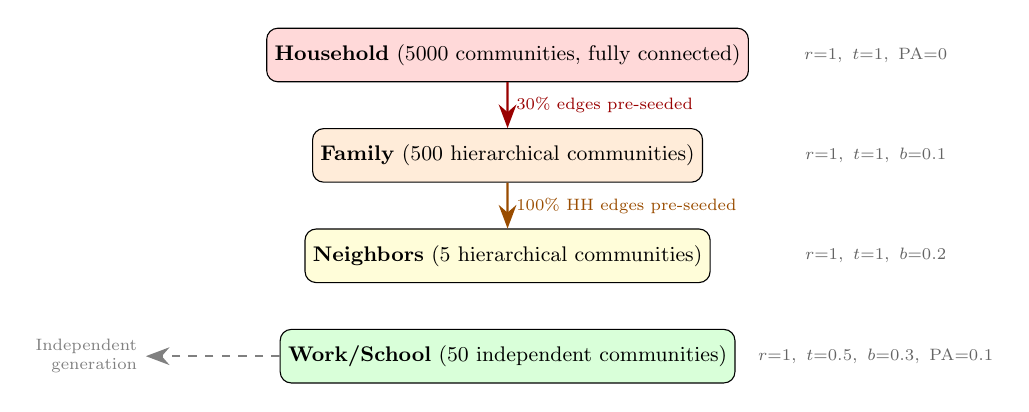
\begin{tikzpicture}[
      layer/.style={draw, rounded corners, minimum width=4cm, minimum height=0.8cm, align=center, font=\small},
      arr/.style={-{Stealth[length=3mm]}, thick},
      scale=0.85, every node/.style={scale=0.85}
    ]
      \node[layer, fill=red!15] (hh) at (0,0) {\textbf{Household} \small(5000 communities, fully connected)};
      \node[layer, fill=orange!15] (fam) at (0,-1.5) {\textbf{Family} \small(500 hierarchical communities)};
      \node[layer, fill=yellow!15] (nb) at (0,-3.0) {\textbf{Neighbors} \small(5 hierarchical communities)};
      \node[layer, fill=green!15] (ws) at (0,-4.5) {\textbf{Work/School} \small(50 independent communities)};

      \draw[arr, red!60!black] (hh) -- node[right, font=\scriptsize] {30\% edges pre-seeded} (fam);
      \draw[arr, orange!60!black] (fam) -- node[right, font=\scriptsize] {100\% HH edges pre-seeded} (nb);
      \draw[arr, gray, dashed] (ws.west) -- ++(-2,0) node[left, font=\scriptsize, align=right] {Independent\\generation};

      % Parameters on the right
      \node[font=\scriptsize, align=left, text=asnugray] at (5.5,-0.0) {$r{=}1,\ t{=}1,\ \text{PA}{=}0$};
      \node[font=\scriptsize, align=left, text=asnugray] at (5.5,-1.5) {$r{=}1,\ t{=}1,\ b{=}0.1$};
      \node[font=\scriptsize, align=left, text=asnugray] at (5.5,-3.0) {$r{=}1,\ t{=}1,\ b{=}0.2$};
      \node[font=\scriptsize, align=left, text=asnugray] at (5.5,-4.5) {$r{=}1,\ t{=}0.5,\ b{=}0.3,\ \text{PA}{=}0.1$};
    \end{tikzpicture}
  \end{center}

  \vspace{0.5em}
  \small Pre-seeding ensures that household members who are also family remain connected in the family layer \textbf{without double-counting} edges against the link budget.
\end{frame}

\begin{frame}{Performance: Rust Backend}
  Critical computation is offloaded to \textbf{Rust} (via PyO3) with automatic Python fallback:

  \vspace{0.5em}
  \begin{table}
    \centering
    \begin{tabular}{@{}l l l@{}}
      \toprule
      \textbf{Operation} & \textbf{Rust Function} & \textbf{Optimization} \\
      \midrule
      Community assignment & \texttt{process\_nodes()} & Vectorized distance computation \\
      Capacity assignment & \texttt{process\_nodes\_capacity()} & Flat 2D arrays, cache-friendly \\
      Edge creation & \texttt{run\_edge\_creation()} & Batch community sampling \\
      \bottomrule
    \end{tabular}
  \end{table}

  \vspace{0.5em}
  \textbf{Key design decisions:}
  \begin{itemize}
    \item Rust provides $10$--$100\times$ speedup over pure Python
    \item All Rust functions have equivalent Python fallbacks for portability
    \item Enables generation at 1\% scale ($\sim$57\,000 nodes) in reasonable time, with path to full-scale
  \end{itemize}
\end{frame}

% ════════════════════════════════════════════════════════════════
%  SECTION 4 — EXPERIMENTS
% ════════════════════════════════════════════════════════════════
\section{Experiments}

\begin{frame}{Experiment 1: Community Structure Analysis}
  \textbf{Setup:} 5\,000 communities generated at 1\% scale ($\sim$57\,000 nodes).

  \vspace{0.5em}
  \begin{columns}[T]
    \begin{column}{0.48\textwidth}
      \textbf{Metrics computed:}
      \begin{itemize}
        \item Community size distribution (mean, std, CV)
        \item Unique groups per community
        \item \textbf{Shannon entropy:}
          $H = -\sum_g p_g \log p_g$
        \item \textbf{Pielou's evenness:}
          $J = H / H_{\max}$
        \item \textbf{Simpson's diversity:}
          $D = 1 - \sum_g p_g^2$
      \end{itemize}
    \end{column}
    \begin{column}{0.50\textwidth}
      \textbf{Key findings:}
      \begin{itemize}
        \item Communities are heterogeneous in size (natural distribution)
        \item Shannon entropy range: 0.0--1.0, indicating variable group diversity within communities
        \item Pielou's evenness: 0.3--0.9, most communities show moderate diversity
        \item Larger communities tend toward higher diversity (size--entropy correlation)
      \end{itemize}
    \end{column}
  \end{columns}

  \vspace{0.5em}
  \small\textit{Visualization: 4-panel plot --- community size distribution, unique groups, Shannon entropy, size vs.\ diversity scatter.}
\end{frame}

\begin{frame}{Experiment 2: Parameter Grid Search}
  \textbf{Setup:} Systematic sweep over community count and preferential attachment strength.

  \vspace{0.3em}
  \begin{columns}[T]
    \begin{column}{0.45\textwidth}
      \textbf{Parameters varied:}
      \begin{itemize}
        \item \textbf{Communities:} 10 values
        \item \textbf{Preferential attachment:} 10 values $\in [0, 1]$
        \item All 4 interaction layers
        \item All characteristic combinations ($2^4 = 16$)
      \end{itemize}

      \vspace{0.5em}
      \textbf{Metrics recorded per network:}
      \begin{itemize}
        \item Number of nodes and edges
        \item Reciprocity
        \item Average clustering coefficient
        \item Degree distribution (mean, std, skewness)
      \end{itemize}
    \end{column}
    \begin{column}{0.52\textwidth}
      \textbf{Key observations:}
      \begin{itemize}
        \item Higher PA $\rightarrow$ more skewed degree distributions (hub formation)
        \item More communities $\rightarrow$ higher clustering within communities
        \item Reciprocity closely tracks the input parameter
        \item Transitivity amplifies clustering beyond the base rate
        \item Different layers produce structurally distinct networks despite same generation engine
      \end{itemize}
    \end{column}
  \end{columns}
\end{frame}

\begin{frame}{Experiment 3: Contagion Dynamics on Generated Networks}
  \textbf{Goal:} Validate that network topology affects diffusion dynamics as expected.

  \vspace{0.3em}
  \begin{columns}[T]
    \begin{column}{0.48\textwidth}
      \textbf{Three contagion models tested:}
      \begin{enumerate}
        \item \textbf{Simple contagion} (SI model)\\
          $P(\text{infect}) = p$ per contact\\
          Parameters: $p{=}0.01$, $I_0{=}800$
        \item \textbf{Complex contagion} (threshold)\\
          Adopt if fraction of infected neighbors $\geq \theta$\\
          Parameters: $\theta{=}0.25$
        \item \textbf{Hybrid contagion}\\
          Heterogeneous thresholds: vulnerable vs.\ normal nodes
      \end{enumerate}

      \vspace{0.3em}
      \small 50 simulations per configuration, vectorized via sparse matrices.
    \end{column}
    \begin{column}{0.50\textwidth}
      \textbf{Results:}
      \begin{itemize}
        \item \textbf{Simple contagion:} Minimal topology dependence --- spreads broadly regardless of structure
        \item \textbf{Complex contagion:} \textit{Highly sensitive} to network topology
          \begin{itemize}
            \item[-] Tightly clustered networks $\rightarrow$ slower spread
            \item[-] Scale-free-like structure $\rightarrow$ faster spread via hubs
          \end{itemize}
        \item \textbf{Variance} in adoption rates correlates with group concentration (Herfindahl index)
      \end{itemize}
    \end{column}
  \end{columns}
\end{frame}

\begin{frame}{Experiment 4: Contagion Parameter Sweep}
  \textbf{Setup:} Threshold sweep ($\theta = 0.05$ to $0.30$) across all network configurations from the grid search.

  \vspace{0.5em}
  \begin{columns}[T]
    \begin{column}{0.55\textwidth}
      \textbf{Design:}
      \begin{itemize}
        \item 5 threshold values $\times$ 10 community counts $\times$ 10 PA values
        \item = 500 network--contagion configurations
        \item Metric: final adoption rate and its variance
      \end{itemize}

      \vspace{0.5em}
      \textbf{Key finding:}
      \begin{block}{Topology--Contagion Interaction}
        The \textbf{variance} in complex contagion outcomes across network realizations is highest for intermediate parameter values --- confirming that ASNU-generated networks produce meaningfully different topologies that affect dynamic processes.
      \end{block}
    \end{column}
    \begin{column}{0.42\textwidth}
      \textbf{Implications:}
      \begin{itemize}
        \item Network structure \textit{matters} for policy-relevant questions (e.g., vaccination strategies)
        \item ASNU's tunable parameters create a rich space of topologies
        \item The choice of PA, community count, and bridge probability produces measurably different diffusion outcomes
      \end{itemize}
    \end{column}
  \end{columns}
\end{frame}

% ════════════════════════════════════════════════════════════════
%  SECTION 5 — RELATED WORK & CONCLUSION
% ════════════════════════════════════════════════════════════════
\section{Comparison \& Conclusion}

\begin{frame}{Comparison with Related Frameworks}
  \begin{table}
    \centering
    \footnotesize
    \begin{tabular}{@{}l c c c c c c@{}}
      \toprule
      & \textbf{Simdemics} & \textbf{June} & \textbf{Jiang+} & \textbf{RTI} & \textbf{FRED} & \cellcolor{asnublue!10}\textbf{ASNU} \\
      \midrule
      Demographic population & \checkmark & \checkmark & \checkmark & \checkmark & \checkmark & \cellcolor{asnublue!10}\checkmark \\
      Network generation & \checkmark & \checkmark & \checkmark & \texttimes & Internal & \cellcolor{asnublue!10}\checkmark \\
      Standalone network tool & \texttimes & \texttimes & Partial & --- & \texttimes & \cellcolor{asnublue!10}\checkmark \\
      Requires geospatial data & \checkmark & \checkmark & \checkmark & \checkmark & \checkmark & \cellcolor{asnublue!10}\texttimes \\
      Multiplex layers & \checkmark & \checkmark & \checkmark & --- & \checkmark & \cellcolor{asnublue!10}\checkmark \\
      Tunable PA / reciprocity & \texttimes & \texttimes & \texttimes & --- & \texttimes & \cellcolor{asnublue!10}\checkmark \\
      Explicit communities & Location & Location & Location & --- & Location & \cellcolor{asnublue!10}\textbf{Agent-based} \\
      Input flexibility & US-specific & UK-specific & US Census & US Census & US Census & \cellcolor{asnublue!10}\textbf{Any CSV} \\
      \bottomrule
    \end{tabular}
  \end{table}

  \vspace{0.5em}
  \textbf{ASNU fills the gap} between:
  \begin{itemize}
    \item Tools that generate \textit{populations without networks} (RTI SynthPop)
    \item Tools that generate \textit{networks inside simulators} (FRED, June)
  \end{itemize}
  \textrightarrow\ A \textbf{standalone}, \textbf{input-flexible}, \textbf{tunable} network generator from aggregate data.
\end{frame}

\begin{frame}{Summary \& Contributions}
  \begin{block}{ASNU: Aggregated Social Network Unfolder}
    A framework for generating realistic synthetic networks from aggregate demographic and interaction data.
  \end{block}

  \vspace{0.5em}
  \textbf{Key contributions:}
  \begin{enumerate}
    \item \textbf{Top-down approach:} Unfolds population-level statistics into individual networks (vs.\ bottom-up rule-based generation)
    \item \textbf{Agent-based community assignment:} Simulated annealing optimizes community composition to match ideal mixing patterns
    \item \textbf{Simultaneously tunable mechanisms:} Preferential attachment, reciprocity, transitivity, and bridge probability operate independently
    \item \textbf{Hierarchical multiplex support:} Layers build upon each other with edge pre-seeding
    \item \textbf{Input agnosticism:} Works with any categorical demographic data --- not tied to a specific country or data source
    \item \textbf{Performance:} Rust backend enables large-scale generation with Python fallback for portability
  \end{enumerate}

  \vspace{0.5em}
  \textbf{Validated through:} community structure analysis, parameter sensitivity studies, and contagion experiments demonstrating that generated network topology meaningfully affects diffusion dynamics.
\end{frame}

\begin{frame}{Future Work}
  \begin{itemize}
    \item \textbf{Weighted edges:} Extend edge creation to support interaction frequency/strength
    \item \textbf{Temporal dynamics:} Generate evolving networks with time-varying interaction patterns
    \item \textbf{Validation against real networks:} Compare generated topological properties with observed contact networks
    \item \textbf{Full-scale generation:} Optimize Rust backend for complete population ($\sim$5.7M nodes)
    \item \textbf{Additional contagion models:} SIR/SEIR dynamics, information diffusion, opinion dynamics
    \item \textbf{Sensitivity analysis:} Systematic study of how input data uncertainty propagates to network properties
  \end{itemize}

  \vspace{1em}
  \begin{center}
    \Large\textbf{Thank you}\\[6pt]
    \normalsize Questions?
  \end{center}
\end{frame}

\end{document}
